\documentclass{manual}

\title{Dual Low-Current Galvanostat}
\author{Blaise J Thompson}

\begin{document}

\maketitle

% TODO: photo of final product

\section{Overview \& Performance}

The dual galvanostat is designed to force a small, constant current through an electrolytic cell.
The voltage floats to whatever is needed to maintain that current.
The maximum rated output voltage is 13 V, although in practice the voltage may be able to float several hundred millivolts above 13.
The positive output (red) is guaranteed to be greater than or equal to the negative return (black), in voltage.
Each output of the dual galvanostat is independent, such that the applied voltages may be different.
However, the current set-point of both outputs is the same.

The dual galvanostat is designed to deliver relatively small currents accurately.
These small current set-points can be crucial when driving particularly slow reactions.
When a galvanostat is set to a current that the reaction of interest cannot support, the galvanostat will naturally swing the output voltage higher.
Often, the galvanostat will end up driving higher-potential undesirable reactions that are more kinetically favorable.
For this reason, this galvanostat has been designed to hold current set-points between 10 $\mu$A and 9.99 mA.

\autoref{fig:setpoint} shows the agreement between the set current and actual measured current for a constant load of 100 $\Omega$.
Note that the data is displayed on a log-log plot.
The output and setpoint agree to within measurement error for all setpoints above 0.30 mA.
Below this setting, however, the agreement worsens---the measured current consistently overshoots the set current.
The absolute deviation between setpoint and measured current never exceeds 30 $\mu$A.
Please note that the galvanostat is still capable of maintaining these low currents.
The displayed value simply may not correspond to the actual current, so an independent calibration is warranted.

\clearpage
\begin{figure}
  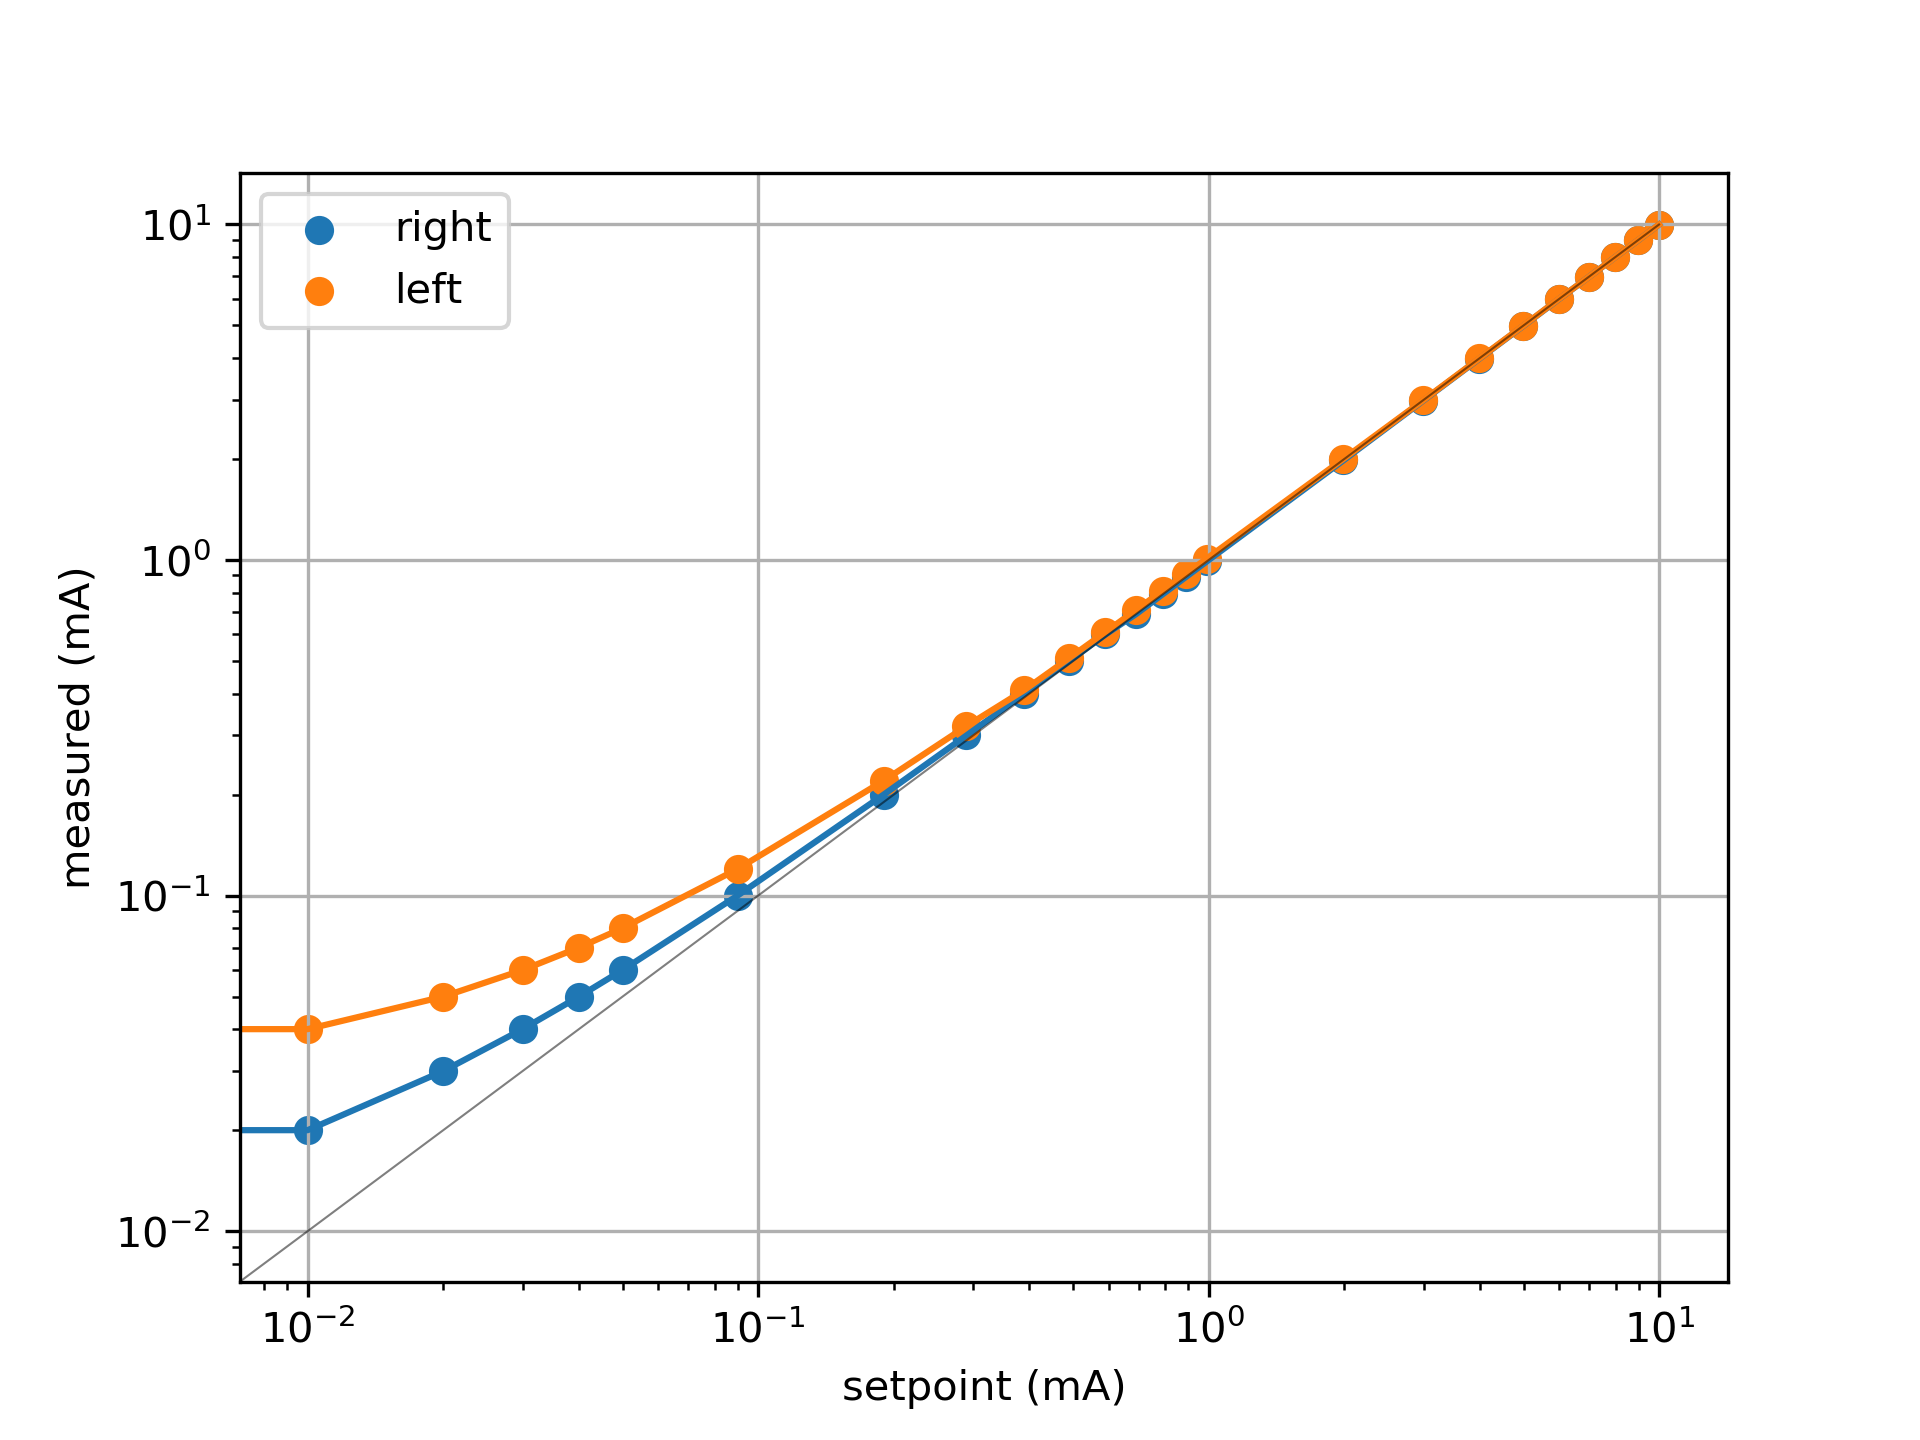
\includegraphics[width=\linewidth]{../data/2018-11-13/setpoint}
  \caption{
    Measured current versus set current.
    On this log-log plot, the entire set-point range of 10 $\mu$A to 9.99 mA can clearly be seen.
    For both outputs, agreement within measurement error is achieved from 0.30 mA to 9.99 mA.
    Unfortunately, both outputs become nonlinear at the lowest setpoints, systematically overshooting the desired current.
    For an unknown reason, the agreement is worse for the left-hand output.
    All readings were taken with a load of 100 $\Omega$.
  }
  \label{fig:setpoint}
\end{figure}
\clearpage

\section{Troubleshooting \& Repair}

\section{Appendix}

This appendix contains the following:
\begin{itemize}
  \item parts list
  \item circuit schematic
  \item full board
  \item top layer
  \item bottom layer
\end{itemize}

\clearpage
\subsection{Parts}

\begin{table}[h]
\begin{tabular}{ l | l | l | l | l }
  name & part & vendor & cost (USD) & comment \\ \hline
  enclosure & Bud XXX & & XXX & \\
  power recepticle & & & & \\
  fuse & & & & \\
  switch & & & & \\
  panel-mount pot & & & & \\
  2x BNC panel mount & & & & \\ \hline
  power supply & & & & \\
  standoffs & & & & \\ \hline
  U1 & LM7905 & UW Stock & 2.00 & TO-220 package \\
  U2 & TI LM311 & \href{https://www.digikey.com/product-detail/en/texas-instruments/LM311N-NOPB/LM311NNS-NOPB-ND/6175}{Digi-Key} & 1.00 & \\
  U3 & TI SN74121N & Digi-Key & & \\
  U4 & TLV4110IP & & & \\
  U5 & INA105KP & & & \\ \hline
  R1 & & & \\
  R2 & & & \\
  R3 & & & \\ \hline
  C1, C2, C3 & 10 $\mu$F electrolytic & UW Stock & 0.25 & must be rated over 15 V\\
  C4 & 10 nF ceramic & UW Stock & 0.25 & \\ \hline
  J1 & Molex 22-23-2031 & UW Stock & 0.25 & 3 pins, 2.54 mm pitch \\
  J2, J3, J4 & Molex 22-23-2021 & UW Stock & 0.25 & 2 pins, 2.54 mm pitch \\
\end{tabular}
\end{table}

Parts list.
Costs are approximate.
Trivial components like screws are not included.

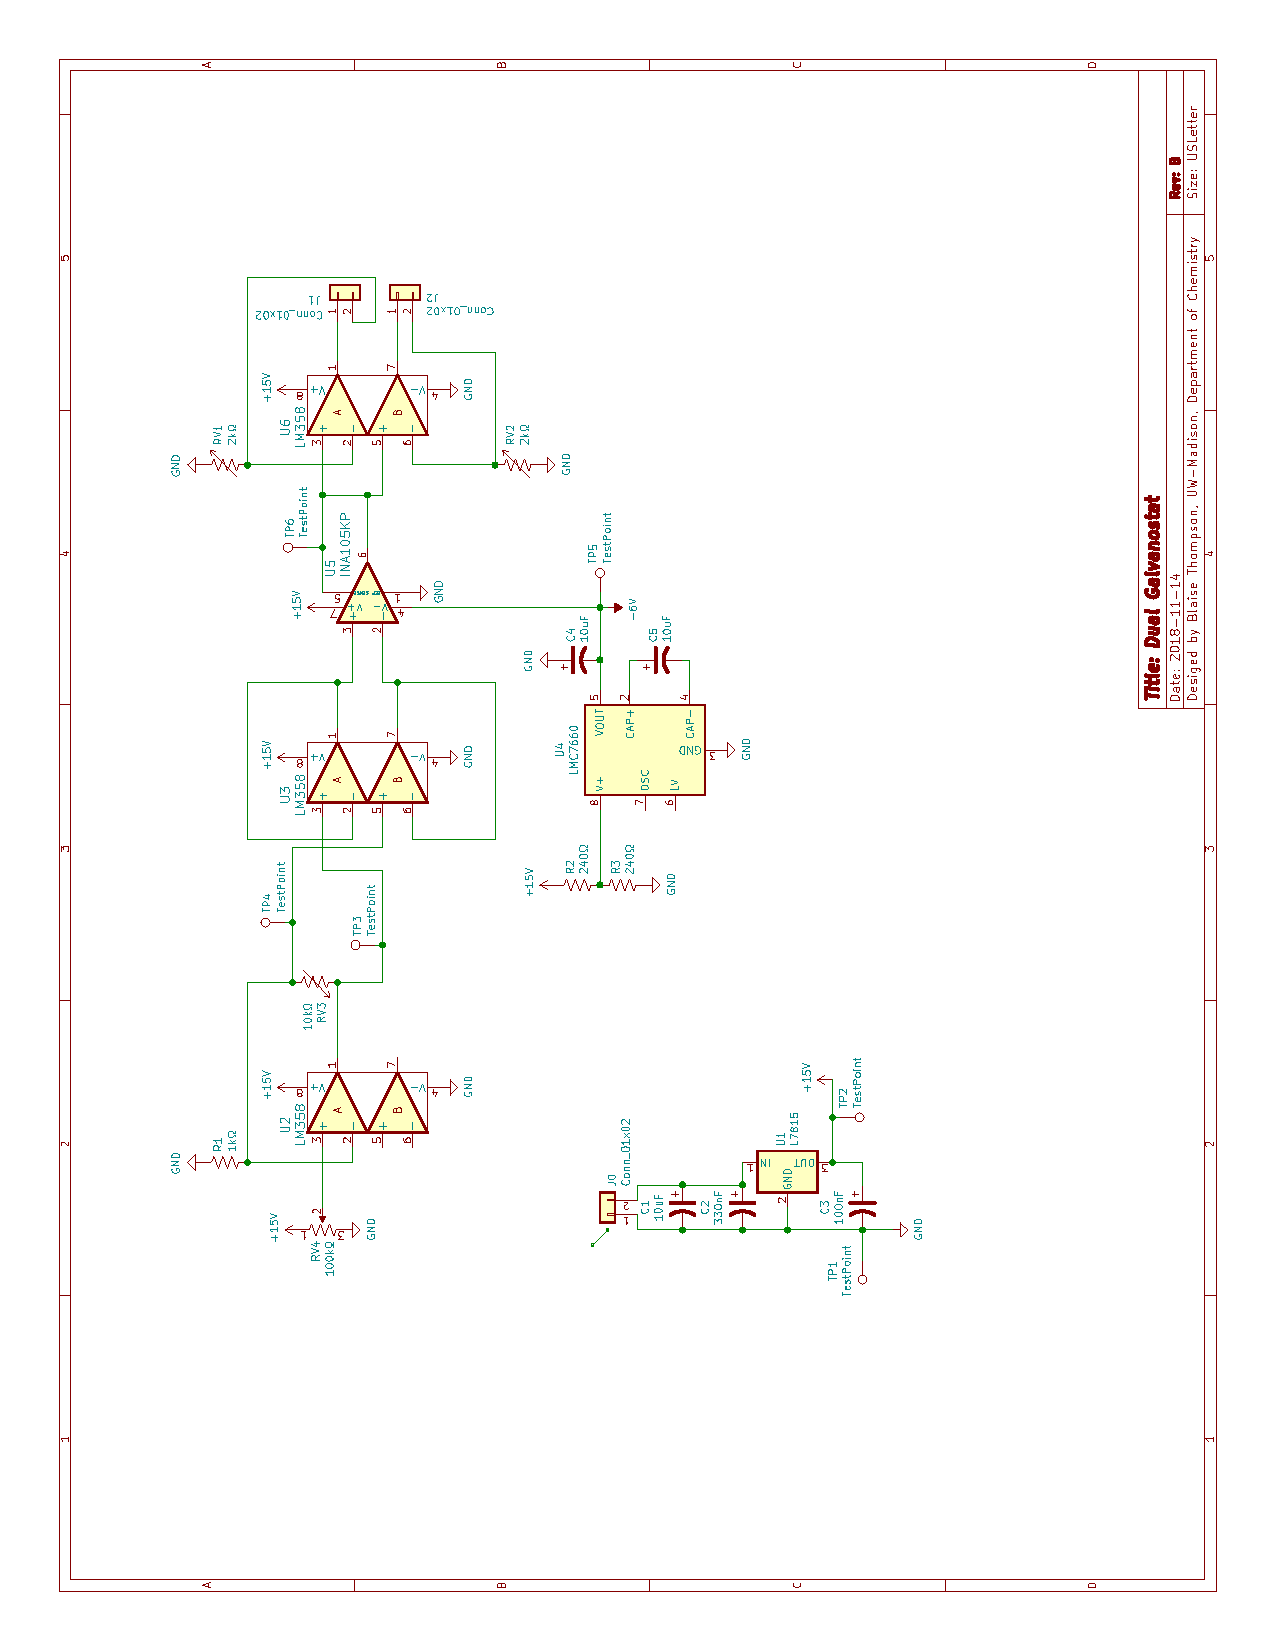
\includepdf[landscape=true]{../PCB/schematic.pdf}
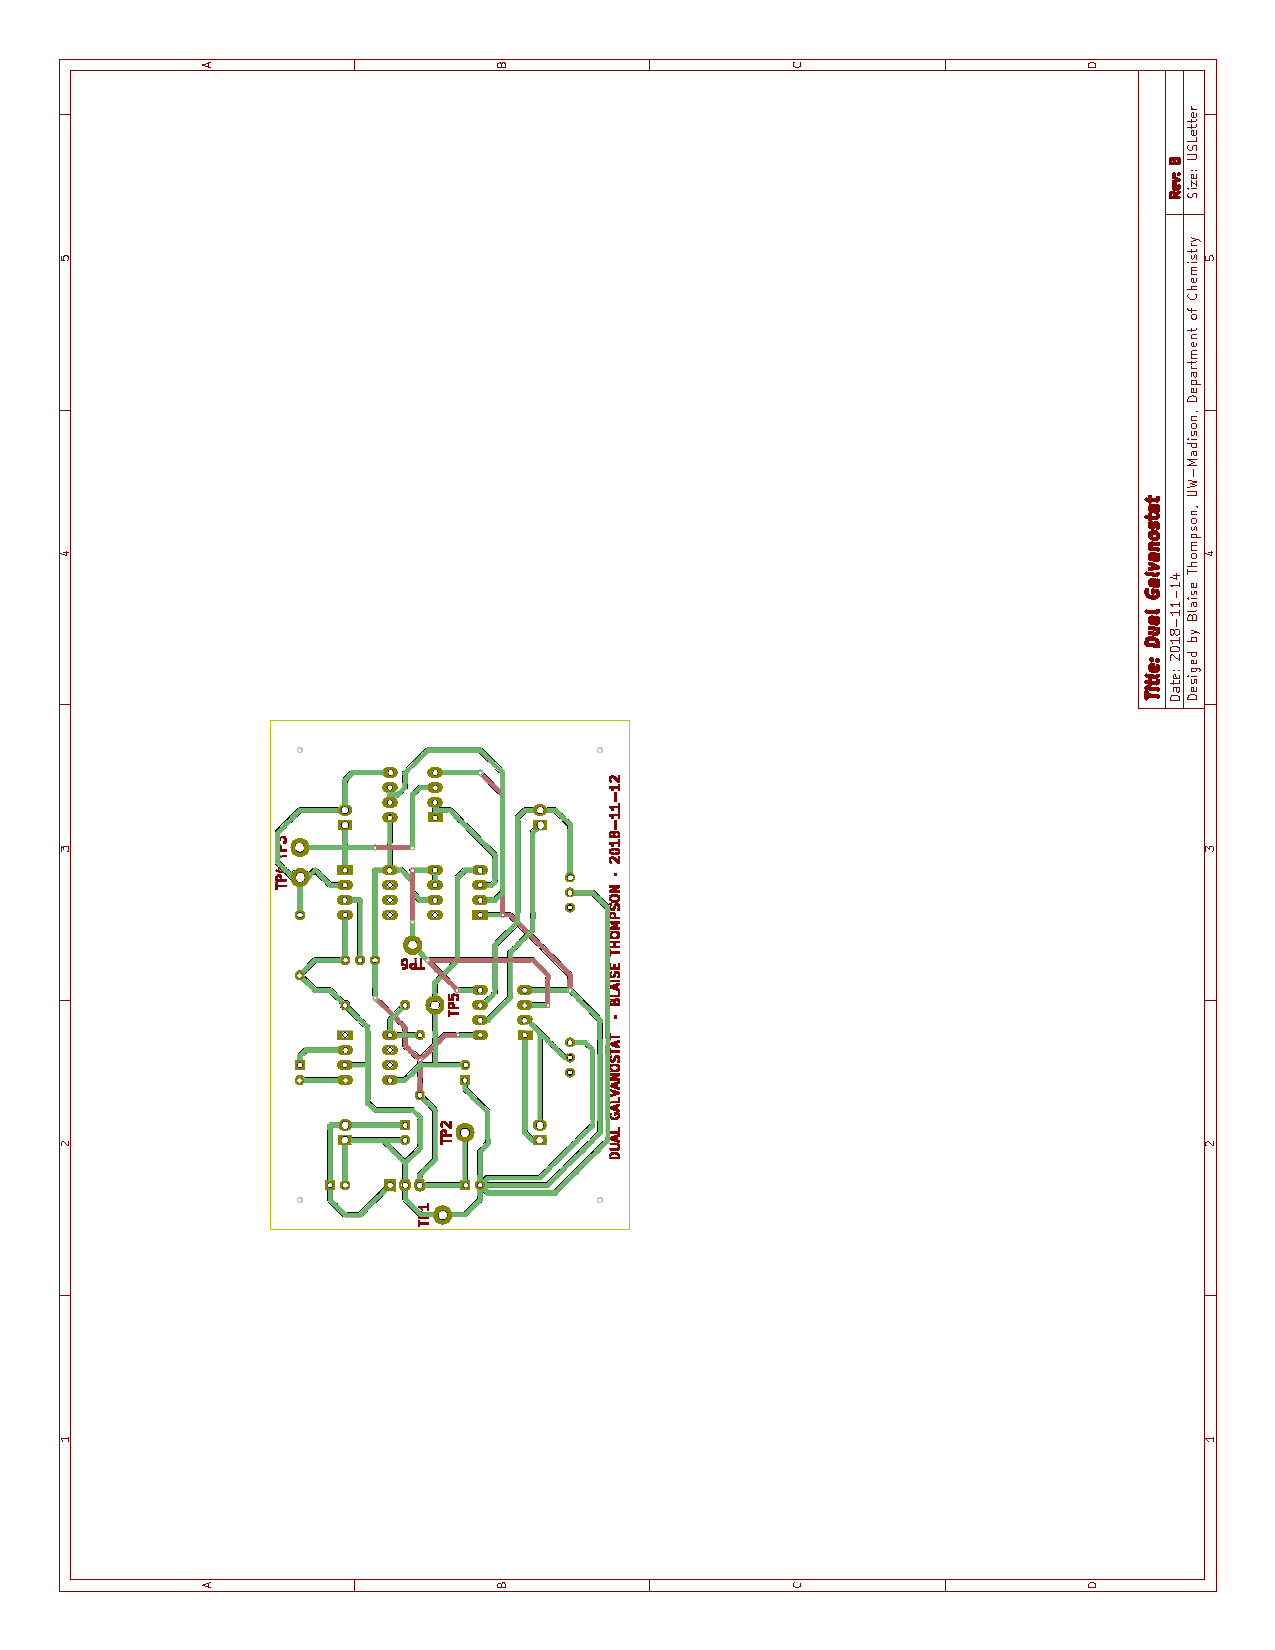
\includepdf{../PCB/pcb.pdf}
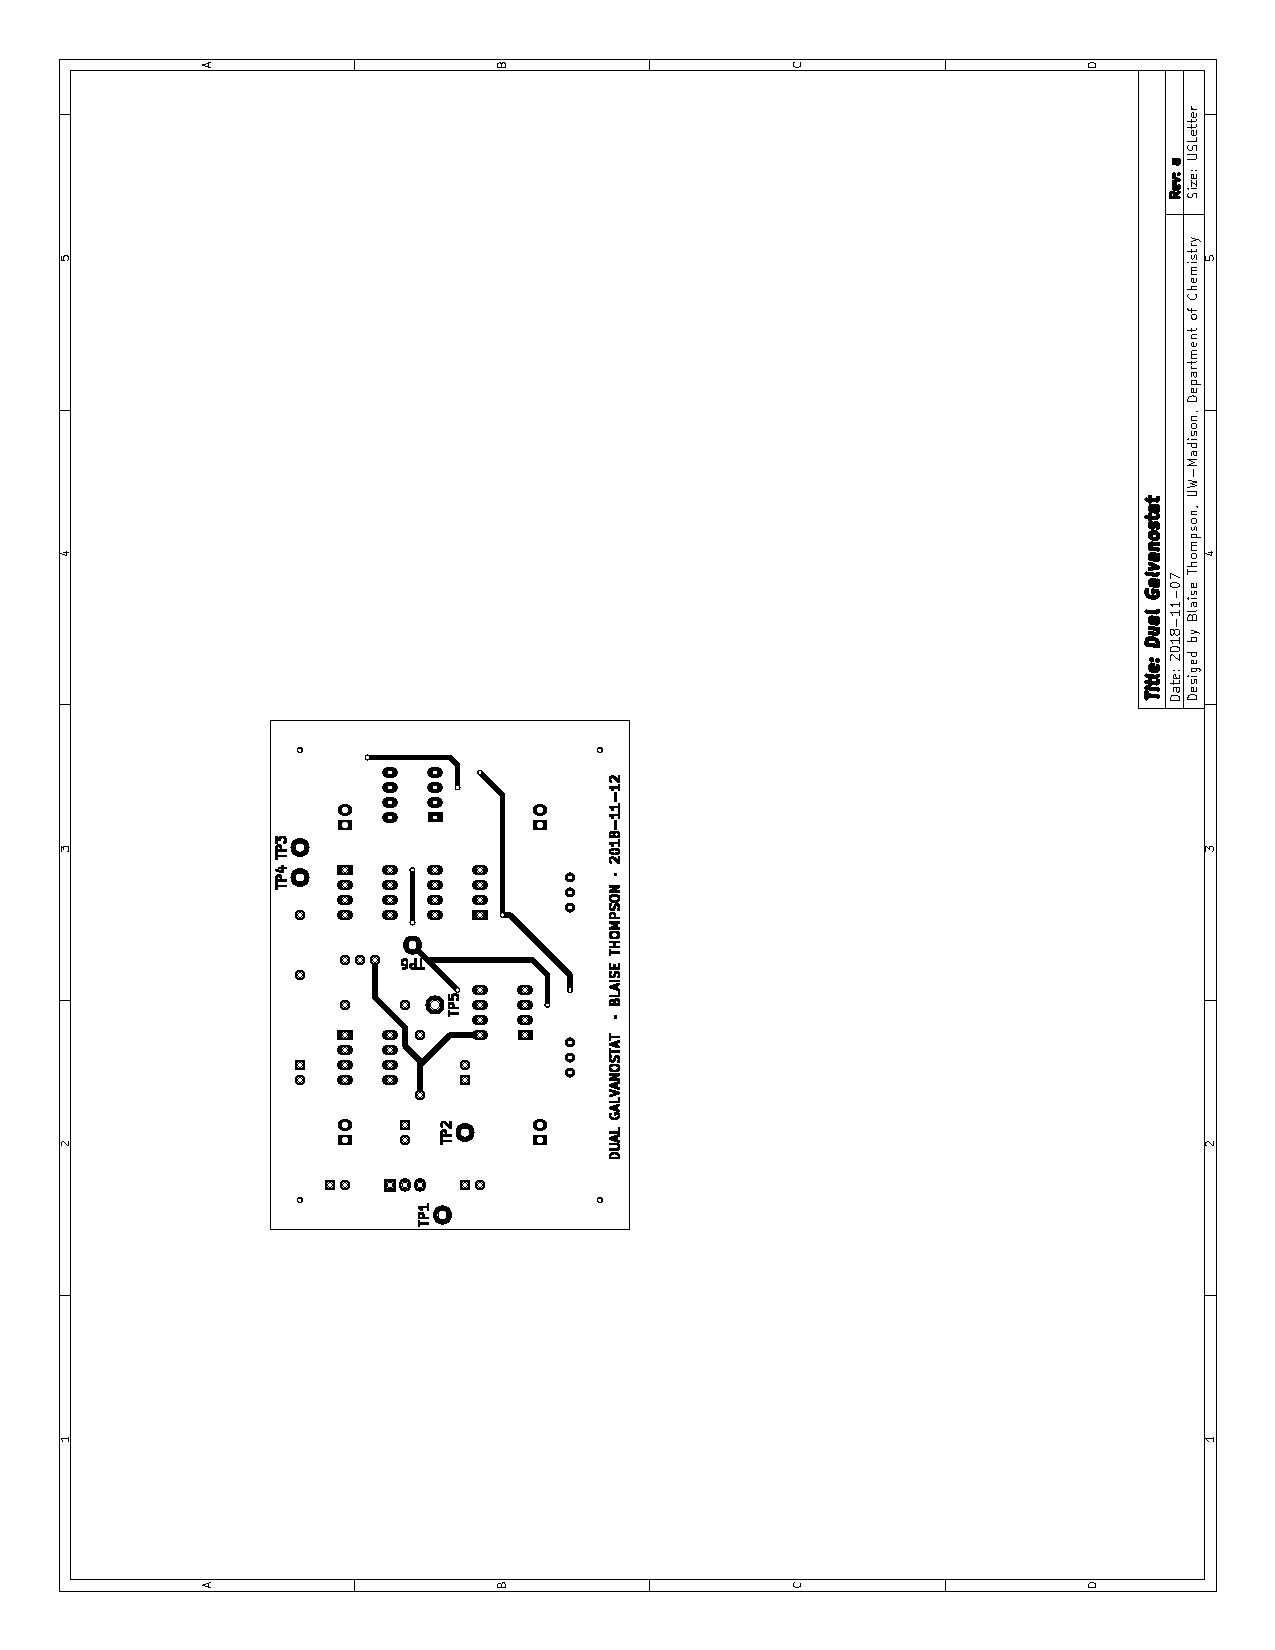
\includepdf{../PCB/front.pdf}
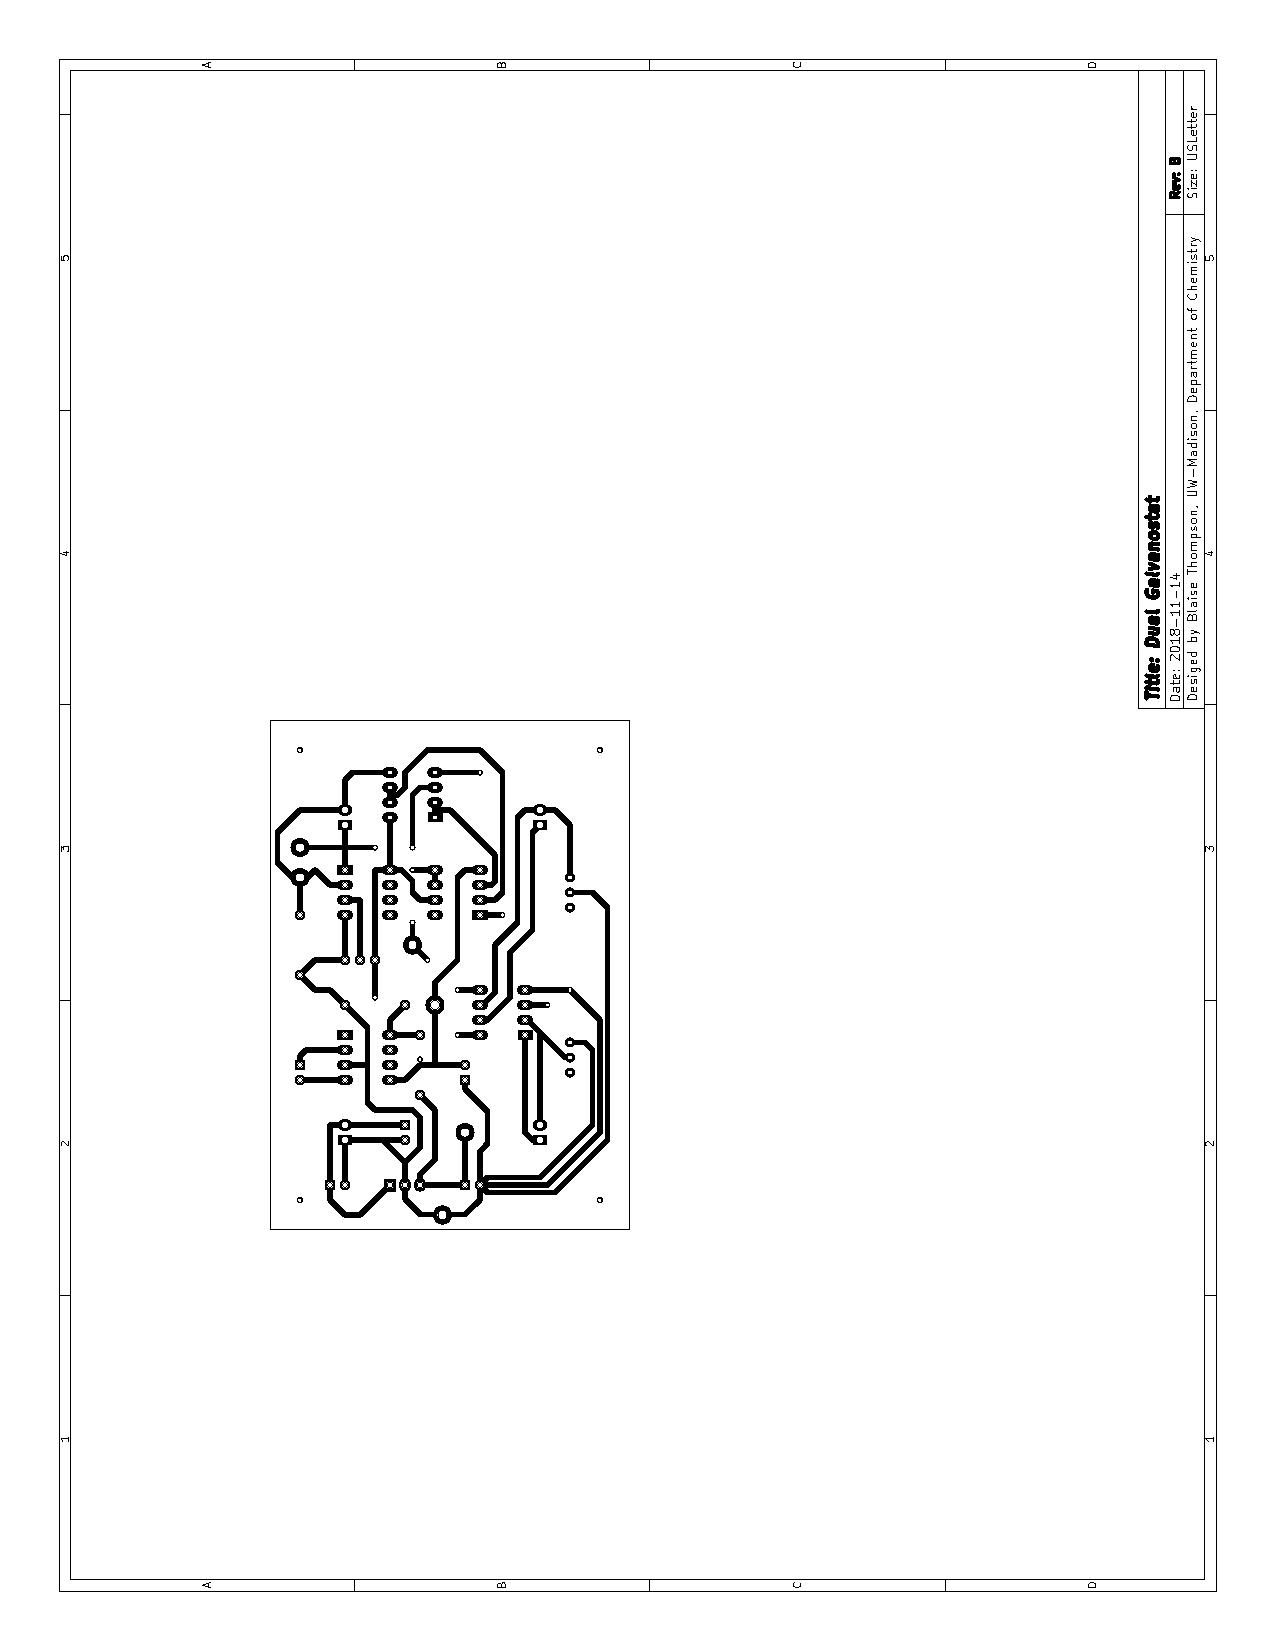
\includepdf{../PCB/back.pdf}

\end{document}
